\documentclass{article}
\usepackage{amsmath}
\usepackage{graphicx}
\begin{document}
\title{Law of Cosines: Question 9}
\author{Ana Bhattacharjee}
\date{\today}
\maketitle{}

\begin{center}
We first need to know that we are working with an equilateral triangle. This means that all the sides are equal to each other. See the visualization below.
\begin{figure}[!htbp]
  \caption{Equilateral Triangle}
  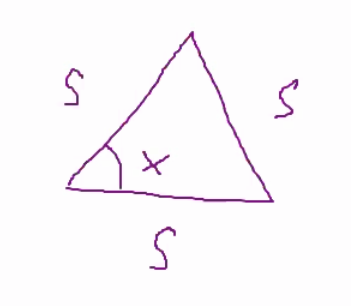
\includegraphics{triangle}
\end{figure}
We can start by setting up the law of cosines for finding angle X.
\begin{align}
s^2 = s^2 + s^2 - 2s^2 cos(x) \\
s^2 = 2s^2 - 2s^2cos(x) \\
s^2 = 2s^2 (1 - cos(x)) \\
\frac{1}{2} = (1 - cos(x))
\end{align}
Using the identity $sin(x) + cos(x) = 1$, we can then substitute the $(1 - cos(x))$ with $sin(x)$ .
\begin{align}
\frac{1}{2} = sin(x) \\
x = sin^{-1}(\frac{1}{2}) \\
x = 60^{\circ}
\end{align}
Since all the sides are equal to s, we can set up the same Law of Cosines equality to find the other two angles and the result for all angles $x^{\circ}$ will be equal to $60^{\circ}$ .  
\end{center}
\end{document}
